\chapter{Resultados}
\label{chap:resultados}

\section{Validação do ambiente e do motor de regras}

Tomando um ambiente em que foram executadas 10.000 simulações de mãos do \textit{Texas Hold'Em}, cada mão sendo repetida 10 vezes, o motor de base 15 executou o trabalho de maneira consistente, classificando todos os jogos de fazer os desempates de maneira correta e robusta. Isso pode ser atestado observando o jogo 20 das simulações, que é o que consta no Apendice-a.

Esta simulação demonstra o funcionamento do motor base 15, já que o \textit{Jogador[0]} e o \textit{Jogador[2]} possuíam dois pares, porém o \textit{Jogador[0]} levou a vitória por pontuar mais, já que, seguindo a fórmula para o motor de desempate, o \textit{jogador[0]} pontuou 2.819.809 pontos, enquanto o \textit{jogador[2]} pontuou 2.819.098, uma diferença de 711 pontos, mesmo o \textit{Jogador[2]} possuindo um kicker de Ás, porém os pares do \textit{jogador[0]} eram superiores.

\section{Evolução na taxa de exploração}

\begin{figure}[htbp]
    \centering
    \caption{Decaimento do fator de exploração \textit{epsilon}($\epsilon$).}
    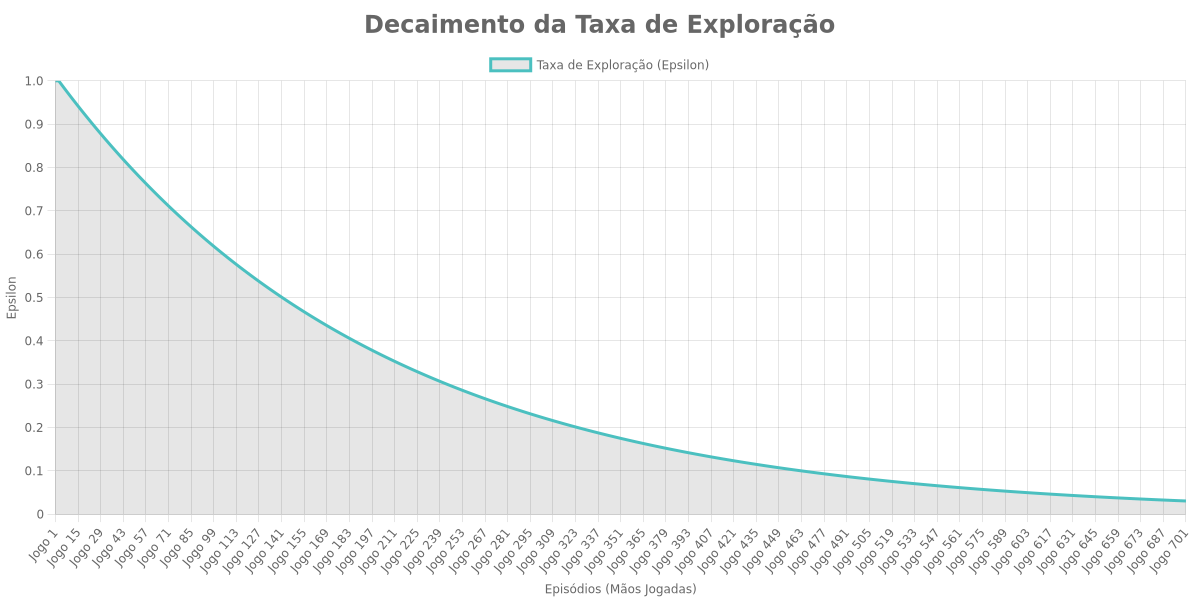
\includegraphics[width=0.8\textwidth]{lib/Decaimento epsilon.png}
    \label{fig:decaimentoEpsilon}

    \small{Fonte: Autoria própria}
\end{figure}

O gráfico demonstra o decaimento do fator de exploração \textit{epsilon} ($\epsilon$), sendo possível notar que a partir de por volta do jogo 700, a taxa de exploração é mínima, significando que o agente está jogando com tudo o que aprendeu, ao invés de apenas tomar ações aleatórias.

\section{Desempenho e lucro do agente}

Durantes as simulações, o agente a ser observado foi o responsável pelo \textit{Jogador[0]}. Para facilitar o entendimento e plotação gráfica, é possível verificar o lucro ou prejuízo do agente observado no seguinte gráfico:

\begin{figure}[htbp]
    \centering
    \caption{Desempenho do agente ao longo das simulações}
    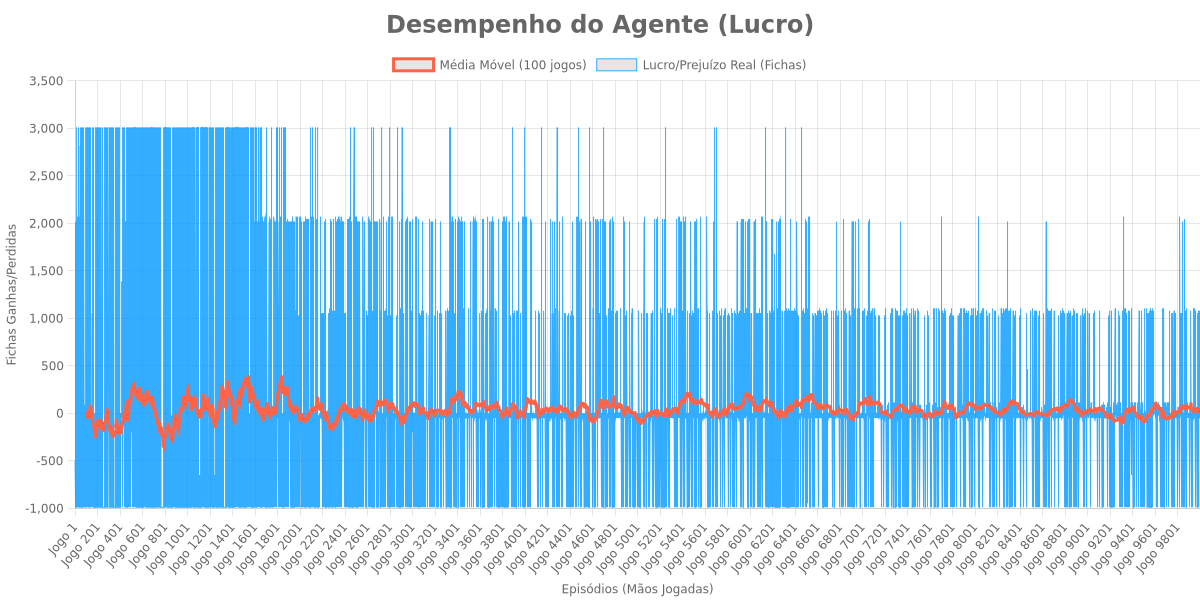
\includegraphics[width=0.97\linewidth]{lib/Desempenho do agente.png}
    \label{fig:desempenhoAgente}

    \small{Fonte: Autoria própria}
\end{figure}

A variância praticamente infinita de estados do \textit{Texas Hold'Em} gera um gráfico com grandes flutuações, porém é possível perceber que a flutuação de ganho e perda de fichas pelo agente cai drasticamente conforme as simulações, as primeiras simulações em que o agente está explorando e toma ações aleatórias a flutuação é maior que nas outras partes, que vão decaindo conforme a rede neural aprende a lidar melhor com os estados.